\documentclass[11pt]{article}
\usepackage{latexsym}
\usepackage{amssymb,amsthm,amsmath}
\usepackage{mathrsfs}
\usepackage[pdftex]{graphicx}
\usepackage{tikz}
\usepackage{pbox}
\usepackage{indentfirst}
\usetikzlibrary{intersections, calc}
\usepackage[margin=1in]{geometry}
\usepackage{listings}

\definecolor{dkgreen}{rgb}{0,0.6,0}
\definecolor{gray}{rgb}{0.5,0.5,0.5}
\definecolor{mauve}{rgb}{0.58,0,0.82}

\lstset{frame=tb,
  language=Python,
  aboveskip=3mm,
  belowskip=3mm,
  showstringspaces=false,
  columns=flexible,
  basicstyle={\small\ttfamily},
  numbers=none,
  numberstyle=\tiny\color{gray},
  keywordstyle=\color{blue},
  commentstyle=\color{dkgreen},
  stringstyle=\color{mauve},
  breaklines=true,
  breakatwhitespace=true,
  tabsize=3
}

\graphicspath{ {figures/} }

\author{{\bf Testing, Testing, 1, 2, 4} \medskip \\ Neil Chainani, Avery Faller, Ed Weng}
\title{CS 181: Machine Learning --- Practical 2}
\date{Friday, March 4, 2016}

\begin{document}

\maketitle

\noindent A given class of malware often has many variants, each of which behaves differently in various contexts. It can be useful, however, to classify malware into broader classes in order to identify potential methods of disinfection. In this paper, we examine how data scientists might automatically classify malware based on logs of system calls made by the malware processes.

\section{Technical Approach}

\subsection{Introduction}
For this exercise, we were given access to 3,086 log files, each of which contain system calls produced by malware executables. Given that we believed certain classes of malware would exhibit similar call patterns, these logs appeared to be good candidates on which to apply classification models. During the process of solving this problem, we made use of Support Vector Machines, Random Forest Classifiers, Logistic Regression, Tensor Flow, Naive Bayes Classifiers, K-Neighbors Classifiers, and Radius Neighbors Classifiers.\\

We discovered that adding counts of system calls as well as adding frequency of various process arguments worked well, increasing our classification accuracy metric significantly from the baseline of 39\%.

\subsection{Data Analysis}
We began this problem by conducting exploratory data analysis on the log files. We started off by examining the distribution of the malware classes \textbf{(Figure \ref{fig:malware_distribution})}. We see that the most common class is "None" followed by "Swizzor" and "VB". Next, we looked at the number of calls made in the log file and looked at the means, standard deviations, maximums, and minimums for each of the 15 classes \textbf{(Figure \ref{fig:length_analysis})}. We did not notice any obvious patterns in the overall call count analysis except that the "Lipler" and "Zbot" had significantly higher means than the other classes.\\

\begin{figure}[t]
\centering
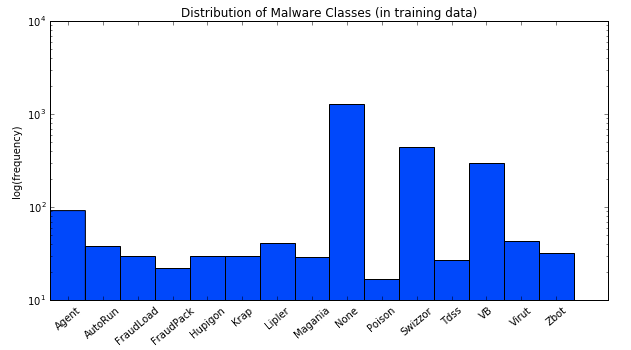
\includegraphics[width=12cm]{malware_distribution}
\caption{Distribution of the malware classes in the full training data set}
\label{fig:malware_distribution}
\vspace{1cm}
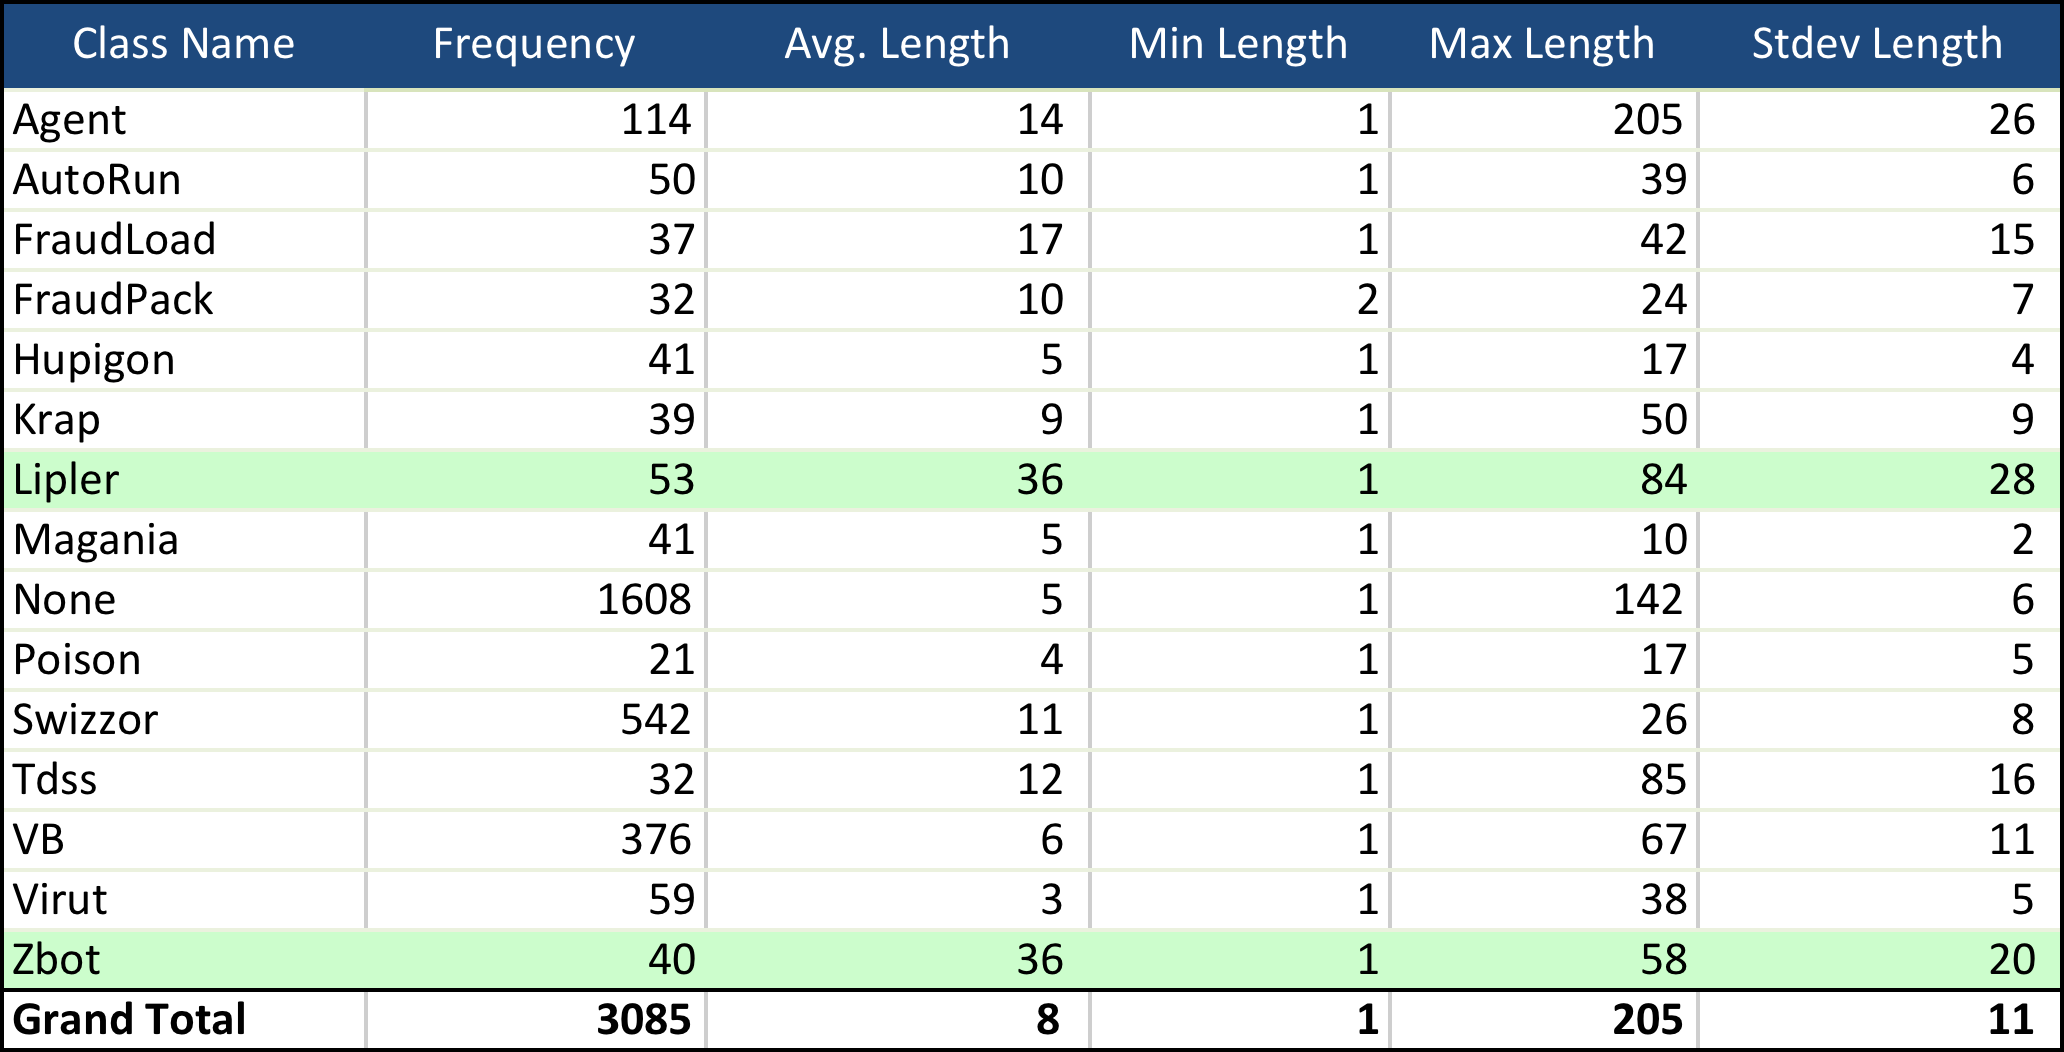
\includegraphics[width=12cm]{length_analysis}
\caption{Statistical analysis performed on overall call counts in training data}
\label{fig:length_analysis}
\end{figure}

Next, we examined the frequency of individual system calls made by specific malware classes. First, we identified 110 different classes of system calls that were shared amongst our test set of log files. We then partitioned our test logs into two groups: a randomly selected training set, which contained 2,468 samples (80\%) and used the remainder as a validation set, which contained 618 samples (20\%). We then used this list of shared system calls to generate frequency tables for the test set, and ran these frequency tables and classification vectors through numerous classification models, such as Support Vector Machines, Random Forest Classifiers, Logistic Regression, Naive Bayes Classifiers, K-Neighbors Classifiers, and Radius Neighbors Classifiers. Of all the models, we found that the Random Forest Classifier worked best on our validation set \textbf{(Figure \ref{fig:model_performance})}.\\

Once we had established that Random Forest Classifiers had the best performance, we began adding features that we thought would increase the efficacy of our model. Features that we added include the process user name argument, the process start reason, and the process termination reason. Adding these three features increased our accuracy by 1.1\%.\\

Next, we attempted to add bi-grams of calls (pairs of consecutive calls) with the idea being that the ordering of calls might reveal certain actions that a class of malware might use to achieve a malicious result. We programmatically generated bi-grams, added them to the feature set, and ran the features through our Random Forest Classifier. Surprisingly, bi-grams did not have a positive effect on our classification accuracy.\\

\begin{figure}[t]
\centering
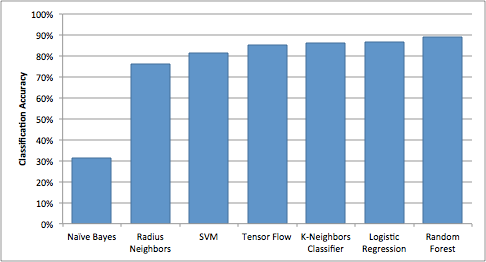
\includegraphics[width=12cm]{model_performance}
\caption{Comparison of model performance on cross-validation data}
\label{fig:model_performance}
\end{figure}

\section{Results}

\begin{figure}[t]
\centering
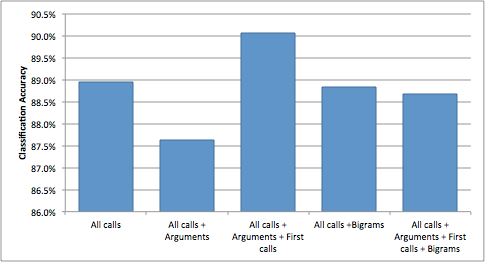
\includegraphics[width=12cm]{result_process}
\caption{Cross-validation results in order of feature additions. Score variance is discussed in the Results section}
\label{fig:result_process}
\end{figure}

\begin{figure}[t]
\centering
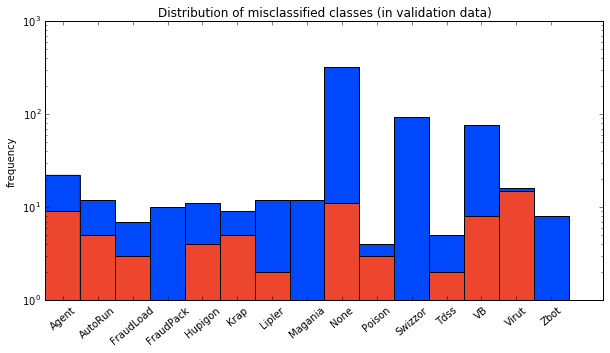
\includegraphics[width=12cm]{misclassified_classes}
\caption{Distribution of misclassified classes using the Random Forest Classifier. Red signifies the misclassified data, while blue signifies the correctly classified data}
\label{fig:misclassified_classes}
\end{figure}

By creating a feature for each call that the executables made, we were able to establish a significant baseline with which to compare our models. We used this feature set to determine which model we would use. Out of all the models that we tried, Random Forest performed the best.  We split our data into training and validation sets and tuned the Random Forest parameters on the validation set.\\

After tuning our Random Forest, we attempted to improve our model by creating more features from the data.  To do this, we inspected the xml files looking for potential features in the xml trees.  Some of the features we extracted from the xml files included the 'username', 'startreason' and 'terminationreason' of the process. These features hurt our accuracy when we added them to the features for the calls. \\

We thought further about what could be used to distinguish between different classes of malware.  We plotted the amount of correctly classified and misclassified data to help us understand if our model had better performance for specific classes of malware \textbf{(Figure \ref{fig:misclassified_classes})}.  While our model was particularly adept at predicting "Swizzor" and "Magania" malware, it fared quite poorly with "Virut", classifying all but one log file incorrectly in our validation test set.\\

Looking into the Virut xml files, we began to think that the order of the first few calls an executable made could be a useful indicator of malware type. Adding the first and second calls of each process's threads improved the performance of our model. When we added the features from above back in, namely 'username', 'startreason' and 'terminationreason', the model further improved overall, but we were still unable to correctly classify "Virut". \\

We then decided to try to capture all orderings of calls in the log files as an extension of the first and second calls, which had worked well.  Adding bi-grams greatly increased the running time of our program as there were an additional 12,100 features in our matrix, but did not increase our accuracy of classification.  In fact, the accuracy dropped as a result of these features, and so we removed them.

\begin{figure}[t]
\centering
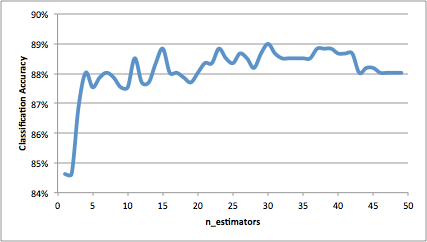
\includegraphics[width=12cm]{n_estimators_tuning}
\caption{Tuning number of trees for Random Forests Classifier}
\label{fig:n_estimators_tuning}

\end{figure}

\section{Discussion}

As we have described above, we began our work by comparing a number of classifiers.  Before tuning this classifiers, Random Forests emerged as the front runner, followed closely by K-Nearest Classifier.  We believe that Random Forests prevailed in this instance because it is a bootstrap method that avoids over-fitting even with small data sets.\\

Generally, a good way to try to improve the accuracy of a classifier is to add more features. However, there were a few instances where this pattern broke down \textbf{(see Figure \ref{fig:result_process})}. One thought we had was that the cross-validation sample was simply too small to yield accurate results during classification scoring. Another thought was that we were severely overfitting to the training data, as we saw a significantly higher classification accuracy on our training data set than we did on our cross-validation data and test data.\\

Another method we tried was introducing bi-grams into our feature set. In order to do so, we counted the number of times certain call pairs appeared in a log file. The intuition here was that we could identify certain types of malware by the frequency with which call pairs were present. We suspect that this intuition was misguided, however, because of the low correlation between the sequencing of the calls and the type of malware that affects it. We also surmised that creating a feature for every single bi-gram, regardless of the rate of occurrence of that bi-gram, introduced more noise and complexity into the model. \\

We also noticed that we were consistently mis-classifying the same malware classes, such as "Virut" and "Agent", across all of the tested models. Our next steps for this practical could include more extensively honing in on the misclassified log files and pinpointing standout features that differ within these classes from the log files of other classes of malware.\\

To account for the large discrepancy between validation accuracy and test accuracy on the Kaggle board, it is important to note the size of our data set. Whereas in the previous practical we had millions of rows, each containing a short string, here we only have a few thousand rows, where each row comprises an entire log file. Since we are training on 2,468 rows and validating on 618 rows, there is a large variance in the efficacy of each model, and we are likely over-fitting. This is the most significant difference between the two practicals that we have had thus far. With more time, we would have performed k-fold cross validation to mitigate these effects. We could also have tried stratified sampling to generate the validation set with proportionally correct malware classes.\\

\section {Code}
\begin{lstlisting}
#
# Github Repo:
# https://github.com/averyfaller/CS181Practical/tree/master/2
#
import os
from collections import Counter
try:
    import xml.etree.cElementTree as ET
except ImportError:
    import xml.etree.ElementTree as ET
import numpy as np
import matplotlib.pyplot as plt

from scipy import sparse
from sklearn import svm
from sklearn.neighbors import KNeighborsClassifier
from sklearn.ensemble import RandomForestClassifier
from sklearn.cross_validation import train_test_split
from sklearn.linear_model import LogisticRegression
from sklearn.gaussian_process import GaussianProcess
from sklearn.naive_bayes import GaussianNB
from sklearn.neighbors import RadiusNeighborsClassifier

TRAIN_DIR = "train"
TEST_DIR = "test"

call_set = set([])

malware_classes = ["Agent", "AutoRun", "FraudLoad", "FraudPack", "Hupigon", "Krap",
           "Lipler", "Magania", "None", "Poison", "Swizzor", "Tdss",
           "VB", "Virut", "Zbot"]

def write_predictions(predictions, ids, outfile):
    """
    assumes len(predictions) == len(ids), and that predictions[i] is the
    index of the predicted class with the malware_classes list above for 
    the executable corresponding to ids[i].
    outfile will be overwritten
    """
    with open(outfile,"w+") as f:
        # write header
        f.write("Id,Prediction\n")
        for i, history_id in enumerate(ids):
            f.write("%s,%d\n" % (history_id, predictions[i]))

def add_to_set(tree):
    for el in tree.iter():
        call = el.tag
        call_set.add(call)

def create_data_matrix(start_index, end_index, direc="train"):
    X = None
    classes = []
    ids = [] 
    i = -1
    for datafile in os.listdir(direc):
        if datafile == '.DS_Store':
            continue

        i += 1
        if i < start_index:
            continue 
        if i >= end_index:
            break

        # extract id and true class (if available) from filename
        id_str, clazz = datafile.split('.')[:2]
        ids.append(id_str)
        # add target class if this is training data
        try:
            classes.append(malware_classes.index(clazz))

        except ValueError:
            # we should only fail to find the label in our list of malware classes
            # if this is test data, which always has an "X" label
            assert clazz == "X"
            classes.append(-1)

        # parse file as an xml document
        tree = ET.parse(os.path.join(direc,datafile))
        add_to_set(tree)
        this_row = call_feats(tree)
        if X is None:
            X = this_row 
        else:
            X = np.vstack((X, this_row))

    return X, np.array(classes), ids

def add_count(feature_dict, feature_name):
    if feature_name not in feature_dict:
        feature_dict[feature_name] = 1
    else:
        feature_dict[feature_name] += 1
    return feature_dict

def call_feats(tree):
    include_other_features = True
    include_first_calls = True
    include_second_calls = True
    include_call_pairs = False

    all_calls = ['recv_socket', 'create_open_file', 'sleep', 'open_scmanager', 'load_driver', 
              'get_host_by_addr', 'create_interface', 'create_mutex', 'set_value', 'enum_items', 
              'get_computer_name', 'read_value', 'write_value', 'change_service_config', 
              'copy_file', 'exit_windows', 'connect_share', 'enum_modules', 'bind_socket', 
              'enum_keys', 'delete_value', 'enum_types', 'open_service', 'processes', 
              'add_share', 'create_socket', 'enum_user', 'dump_line', 'unload_driver', 
              'enum_values', 'thread', 'load_dll', 'create_window', 'read_section_names', 
              'com_create_instance', 'message', 'get_userinfo', 'get_file_attributes', 'find_file', 
              'open_file', 'get_username', 'create_service', 'query_value', 'create_file', 
              'move_file', 'open_key', 'send_socket', 'vm_write', 'delete_file', 
              'create_process_as_user', 'get_system_time', 'create_mailslot', 'com_createole_object', 
              'listen_socket', 'enum_share', 'open_mutex', 'vm_protect', 'all_section', 
              'vm_mapviewofsection', 'get_windows_directory', 'enum_processes', 'open_url', 
              'download_file', 'com_get_class_object', 'kill_process', 'load_image', 'delete_share', 
              'create_process', 'logon_as_user', 'get_system_directory', 'set_thread_context', 
              'create_process_nt', 'destroy_window', 'vm_allocate', 'enum_handles', 'connect_socket', 
              'set_file_time', 'start_service', 'create_thread_remote', 'show_window', 'open_process', 
              'impersonate_user', 'connect', 'enum_services', 'process', 'vm_read', 'check_for_debugger', 
              'query_keyinfo', 'delete_service', 'read_section', 'enum_window', 'set_system_time', 
              'add_netjob', 'ping', 'set_windows_hook', 'control_service', 'accept_socket', 
              'trimmed_bytes', 'download_file_to_cache', 'find_window', 'get_host_by_name', 
              'set_file_attributes', 'revert_to_self', 'create_key', 'create_thread', 'enum_subtypes', 
              'delete_key', 'create_directory', 'remove_directory', 'create_namedpipe']

    first_calls = map(lambda call: "fc_" + call, all_calls)

    second_calls = map(lambda call: "sc_" + call, all_calls)

    call_pairs = map(lambda call_one: map(lambda call_two: call_one + "_" + call_two, second_calls), first_calls)

    all_features = all_calls

    if include_other_features:
        other_features = ['Administrator', 'SYSTEM', 'NETZWERKDIENST', 'LOKALER DIENST', 
                      'SCM', 'InjectedCode', 'SvcHost', 'CreateProcess', 'BHOInstalled', 'DCOMService', 'AnalysisTarget',
                     'NormalTermination', 'Unknown', 'KilledByWindowsLoader', 'Timeout']
        all_features += other_features
    if include_first_calls:
        all_features += first_calls
    if include_second_calls:
        all_features += second_calls
    if include_call_pairs:
        all_features += call_pairs

    feature_dict = {}
    last_call='start'
    for el in tree.iter():
        call = el.tag
        feature_dict = add_count(feature_dict, call)
    
    # Attempt to add arguments of username, startreason, and terminationreason
    if include_other_features:
        root = tree.getroot()
        for process in root.findall('process[@username]'):
            username = process.attrib['username']
            feature_dict = add_count(feature_dict, username)
        for process in root.findall('process[@startreason]'):
            startreason = process.attrib['startreason']
            feature_dict = add_count(feature_dict, startreason)
        for process in root.findall('process[@terminationreason]'):
            terminationreason = process.attrib['terminationreason']
            feature_dict = add_count(feature_dict, terminationreason)

    # Attempt to add first and second calls
    j = 0
    for call in root.findall('process/thread/all_section/'):
        name = call.tag
        if (name != 'load_image') and (name != 'load_dll'): 
            j += 1
            if include_first_calls and j == 1:
                first_call = 'fc_' + name
                feature_dict = add_count(feature_dict, first_call)
            if include_second_calls and j == 2:
                second_call = 'sc_' + name
                feature_dict = add_count(feature_dict, second_call)
                break
    
    # Attempt to add call-pairs, which, in theory, help account for sequencing of calls.
    # This perhaps should be extended to call-triplets, etc.
    if include_call_pairs:
        for idx, call in enumerate(root.findall('process/thread/all_section/')):
            if idx == 1:
                second_call = call.tag
            elif idx >= 2:
                first_call = second_call
                second_call = call.tag
                call_pair = "fc_" + first_call + "_sc_" + second_call
                feature_dict = add_count(feature_dict, call_pair)
            
    call_feat_array = np.zeros(len(all_features))
    for i in range(len(all_features)):
        call = all_features[i]
        call_feat_array[i] = 0
        if call in feature_dict:
            call_feat_array[i] = feature_dict[call]

    return call_feat_array

def write_to_file(filename, ids, predictions):
    zips = zip(ids, predictions)
    with open(filename, "w") as f:
        f.write("Id,Prediction\n")
        for i,p in enumerate(zips):
            f.write(str(p[0]) + "," + str(p[1]) + "\n")

def main():
    X_train_all, t_train_all, train_all_ids = create_data_matrix(0, 3086, TRAIN_DIR)
    X_train, X_valid, t_train, t_valid = train_test_split(X_train_all, t_train_all, test_size=0.20, random_state=37)
    X_test_all, t_test_all, test_all_ids = create_data_matrix(0, 3724, TEST_DIR)

    print X_train.shape
    print X_valid.shape
    
    sv = svm.SVC(kernel='poly')
    sv.fit(X_train, t_train)
    print "SVM Score was: %f" % clf.score(X_valid, t_valid)

    rf = RandomForestClassifier(n_estimators=30, min_samples_split=1, random_state=37)
    rf.fit(X_train, t_train)
    print "RandomForest Score was: %f" % (rf.score(X_valid, t_valid))

    lr = LogisticRegression(penalty='l2',solver='newton-cg',max_iter=500)
    lr.fit(X_train, t_train)
    print "LogisticRegression Score was: %f" % (lr.score(X_valid, t_valid))

    clf = GaussianNB()
    clf.fit(X_train, t_train)
    print "GaussianNB Score was: %f" % (clf.score(X_valid, t_valid))

    nn = KNeighborsClassifier(n_neighbors=6, weights='uniform')
    nn.fit(X_train, t_train)
    score = nn.score(X_valid, t_valid)
    print "KNeighbors Score was: %f" % (score)

    rnc = RadiusNeighborsClassifier(radius=6,outlier_label=8, p=2)
    rnc.fit(X_train, t_train)
    print "RadiusNeighbors Score was: %f" % (rnc.score(X_valid, t_valid))

    # Get predictions
    rf = RandomForestClassifier(n_estimators=30, min_samples_split=1)
    rf.fit(X_train_all, t_train_all)
    test_predictions = rf.predict(X_test_all)

    write_to_file("prediction.csv", test_all_ids, test_predictions)

if __name__ == "__main__":
    main()
\end{lstlisting}

\end{document}